
%(BEGIN_QUESTION)
% Copyright 2014, Tony R. Kuphaldt, released under the Creative Commons Attribution License (v 1.0)
% This means you may do almost anything with this work of mine, so long as you give me proper credit

This pictorial diagram shows the wiring connections for a simple pressure control loop, where a loop-powered 4-20 mA pressure transmitter sends a signal to a Honeywell controller, which in turn sends another 4-20 mA signal to a control valve:

$$\includegraphics[width=15.5cm]{i01298x01.eps}$$

Suppose the operator informs you that the control valve refuses to open, no matter what value she sets the output of the controller in manual mode.  Your job now is to diagnose the problem in this control loop using only basic test equipment (e.g. digital multimeter, hand tools).

Determine the diagnostic value of each of the following tests.  Assume only one fault in the system, including any single component or any single wire/cable/tube connecting components together.  If a proposed test could provide new information to help you identify the location and/or nature of the one fault, mark ``yes.''  Otherwise, if a proposed test would not reveal anything relevant to identifying the fault (already discernible from the measurements and symptoms given so far), mark ``no.''

% No blank lines allowed between lines of an \halign structure!
% I use comments (%) instead, so that TeX doesn't choke.

$$\vbox{\offinterlineskip
\halign{\strut
\vrule \quad\hfil # \ \hfil & 
\vrule \quad\hfil # \ \hfil & 
\vrule \quad\hfil # \ \hfil \vrule \cr
\noalign{\hrule}
%
% First row
{\bf Diagnostic test} & {\bf Yes} & {\bf No} \cr
%
\noalign{\hrule}
%
% Another row
Place controller in automatic mode &  &  \cr
%
\noalign{\hrule}
%
% Another row
Measure $V_{AB}$ with controller output set to 100\% (manual mode) &  &  \cr
%
\noalign{\hrule}
%
% Another row
Measure $V_{5-4}$ with controller output set to 100\% (manual mode) &  &  \cr
%
\noalign{\hrule}
%
% Another row
Measure $V_{8-7}$ with controller output set to 50\% (manual mode) &  &  \cr
%
\noalign{\hrule}
%
% Another row
``Crack'' open tube fitting at the ``S'' port on the I/P transducer &  &  \cr
%
\noalign{\hrule}
%
% Another row
``Crack'' open tube fitting at the ``O'' port on the I/P transducer &  &  \cr
%
\noalign{\hrule}
%
% Another row
Press the I/P transducer's flapper closer to its nozzle &  &  \cr
%
\noalign{\hrule}
%
% Another row
Pull the I/P transducer's flapper away from its nozzle &  &  \cr
%
\noalign{\hrule}
%
% Another row
Tighten the nuts compressing the control valve's stem packing &  &  \cr
%
\noalign{\hrule}
%
% Another row
Loosen the nuts compressing the control valve's stem packing &  &  \cr
%
\noalign{\hrule}
%
% Another row
Measure the output voltage of the DC power supply &  &  \cr
%
\noalign{\hrule}
%
% Another row
Measure voltage across the pressure transmitter terminals &  &  \cr
%
\noalign{\hrule}
%
% Another row
Measure voltage across the I/P transducer terminals &  &  \cr
%
\noalign{\hrule}
} % End of \halign 
}$$ % End of \vbox

\underbar{file i01298}
%(END_QUESTION)





%(BEGIN_ANSWER)

% No blank lines allowed between lines of an \halign structure!
% I use comments (%) instead, so that TeX doesn't choke.

$$\vbox{\offinterlineskip
\halign{\strut
\vrule \quad\hfil # \ \hfil & 
\vrule \quad\hfil # \ \hfil & 
\vrule \quad\hfil # \ \hfil \vrule \cr
\noalign{\hrule}
%
% First row
{\bf Diagnostic test} & {\bf Yes} & {\bf No} \cr
%
\noalign{\hrule}
%
% Another row
Place controller in automatic mode &  & $\surd$ \cr
%
\noalign{\hrule}
%
% Another row
Measure $V_{AB}$ with controller output set to 100\% (manual mode) &  & $\surd$ \cr
%
\noalign{\hrule}
%
% Another row
Measure $V_{5-4}$ with controller output set to 100\% (manual mode) & $\surd$ &  \cr
%
\noalign{\hrule}
%
% Another row
Measure $V_{8-7}$ with controller output set to 50\% (manual mode) &  & $\surd$ \cr
%
\noalign{\hrule}
%
% Another row
``Crack'' open tube fitting at the ``S'' port on the I/P transducer & $\surd$ &  \cr
%
\noalign{\hrule}
%
% Another row
``Crack'' open tube fitting at the ``O'' port on the I/P transducer & $\surd$ &  \cr
%
\noalign{\hrule}
%
% Another row
Press the I/P transducer's flapper closer to its nozzle & $\surd$ &  \cr
%
\noalign{\hrule}
%
% Another row
Pull the I/P transducer's flapper away from its nozzle &  & $\surd$ \cr
%
\noalign{\hrule}
%
% Another row
Tighten the nuts compressing the control valve's stem packing &  & $\surd$ \cr
%
\noalign{\hrule}
%
% Another row
Loosen the nuts compressing the control valve's stem packing &  & ? \cr
%
\noalign{\hrule}
%
% Another row
Measure the output voltage of the DC power supply &  & $\surd$ \cr
%
\noalign{\hrule}
%
% Another row
Measure voltage across the pressure transmitter terminals &  & $\surd$ \cr
%
\noalign{\hrule}
%
% Another row
Measure voltage across the I/P transducer terminals & $\surd$ &  \cr
%
\noalign{\hrule}
} % End of \halign 
}$$ % End of \vbox

Loosening the nuts on the control valve's stem packing is a questionable test because control valve actuators generally exert sufficient force to overcome even the worst cases of stem packing friction.  Thus, it is highly unlikely that stem packing friction is the cause of the valve's unresponsiveness, and as such this test should be avoided unless it is determined that the valve actuating diaphragm is indeed receiving full air pressure from the I/P.
 
%(END_ANSWER)





%(BEGIN_NOTES)


%INDEX% Pictorial circuit review (4-20 mA loop)
%INDEX% Troubleshooting review: electric circuit diagnostic test usefulness
%INDEX% Troubleshooting review: electric circuits

%(END_NOTES)


